\documentclass[conference]{IEEEtran}
\IEEEoverridecommandlockouts
% The preceding line is only needed to identify funding in the first footnote. If that is unneeded, please comment it out.
\usepackage{cite}
\usepackage{amsmath,amssymb,amsfonts}
\usepackage{algorithmic}
\usepackage{graphicx}
\usepackage{textcomp}
\usepackage{xcolor}
\usepackage{listings}
\usepackage{pgfplotstable}

\def\BibTeX{{\rm B\kern-.05em{\sc i\kern-.025em b}\kern-.08em
    T\kern-.1667em\lower.7ex\hbox{E}\kern-.125emX}}
\begin{document}

\title{Extended Generative Adversarial Networks}

\author{\IEEEauthorblockN{John Hancock}
\IEEEauthorblockA{\textit{College of Engineering and Computer Science} \\
\textit{Florida Atlantic University}\\
Boca Raton, United States of America\\
jhancoc4@fau.edu}}


\maketitle

\begin{abstract}
In this work we explore extending generative adversarial networks (GAN's). Authors of 
previous research document GAN's with one generator and one discriminator. In
this work we explore GAN's with more than one generator or discriminator, and
we investigate the performance of these extended GAN's.
\end{abstract}

\begin{IEEEkeywords}
generative adversarial networks, gan, neural networks, deep learning
\end{IEEEkeywords}

\section{Introduction}

\section{Related Work}

\section{Chained Generative Adversarial Networks}
\begin{figure}[htpb]
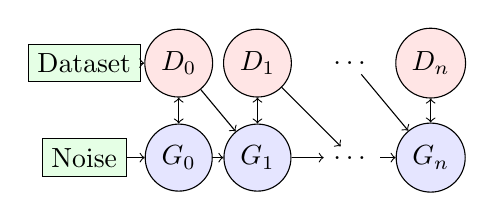
\begin{tikzpicture}
%style for generator node
\tikzstyle{gnode} = [circle, fill=blue!10, draw=black]

%style for discriminator node
\tikzstyle{dnode} = [circle, fill=red!10, draw=black]

%style for input box
\tikzstyle{inbox} = [rectangle, fill=green!10, draw=black]

%place nodes
\node[gnode](G0) at (0,0) {$G_{0}$};
\node[dnode](D0) at (0,1.2) {$D_{0}$};
\node[inbox](noise) at (-1.2,0) {Noise};
\node[inbox](dataset) at (-1.2,1.2) {Dataset};
\node[gnode](G1) at (1,0) {$G_{1}$};
\node[dnode](D1) at (1, 1.2) {$D_{1}$};
\node(upperDots) at (2.2,1.2){\ldots};
\node(lowerDots) at (2.2,0){\ldots};
\node[gnode](GN) at (3.2,0) {$G_{n}$};
\node[dnode](DN) at (3.2, 1.2) {$D_{n}$};

%connect nodes with lines
\draw[->] (noise)-- (G0);
\draw[->] (dataset)-- (D0);
\draw[<->] (G0) -- (D0);
\draw[->] (G0) -- (G1);
\draw[->] (D0) -- (G1);
\draw[<->] (G1) -- (D1);
\draw[->] (G1) -- (lowerDots);
\draw[->] (D1) -- (lowerDots);
\draw[->] (lowerDots) -- (GN);
\draw[->] (upperDots) -- (GN);
\draw[<->] (DN) -- (GN);
\end{tikzpicture}
\caption{Chained GANs architecture}
\label{figCGANHigh}
\end{figure}

% diagram of base GAN
\begin{figure}[htpb]
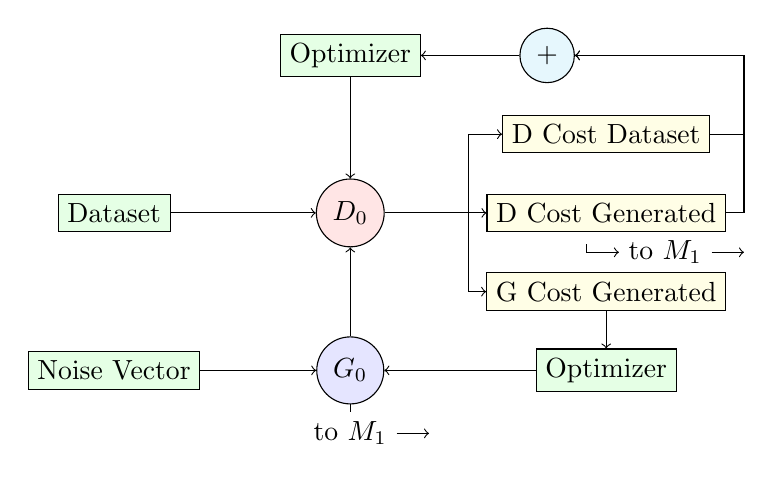
\begin{tikzpicture}
%style for generator node
\tikzstyle{gnode} = [circle, fill=blue!10, draw=black]

%style for discriminator node
\tikzstyle{dnode} = [circle, fill=red!10, draw=black]

%style for input box
\tikzstyle{inbox} = [rectangle, fill=green!10, draw=black]

%style for cost 
\tikzstyle{cost} = [rectangle, fill=yellow!10, draw=black]

%style for operator 
\tikzstyle{operator} = [circle, fill=cyan!10, draw=black]

%place nodes
\node[inbox] (noise) at (0,0) {Noise Vector};

\node[inbox] (dataset) at (0,2) {Dataset};

\node[gnode](generator) at (3,0) {$G_{0}$};

\node(gIToNext) at (3,-0.8) {to $M_{1}$}; 

\node[inbox] (gOptimizer) at (6.25, 0) {Optimizer};

\node[dnode](discriminator) at (3,2) {$D_{0}$};

\node[inbox] (dOptimizer) at (3,4) {Optimizer};

\node[cost] (dCostDataset) at (6.25,3){D Cost Dataset};

\node[cost] (dCostGenerated) at (6.25,2){D Cost Generated};
\node (dItoNext) at (7.0, 1.5){to $M_{1}$};

\node[cost] (gCostGenerated) at (6.25,1){G Cost Generated};

\node[operator] (adder) at (5.5,4){+};

\draw[->] (noise) -- (generator);

\draw[->] (generator) -- (discriminator) ;
\draw[->] (generator) -- (gIToNext) -- (4,-0.8);

\draw[->] (gOptimizer) -- (generator);

\draw[->] (gCostGenerated) -- (gOptimizer);

\draw[->] (dataset) -- (discriminator);

\draw[->] (discriminator) -- (4.5, 2) |- (dCostDataset);
\draw[->] (discriminator) -- (4.5,2) |- (gCostGenerated);
\draw[->] (dCostGenerated) (6.0,1.6) |- (6.0,1.5) |- (dItoNext);
\draw[->] (dItoNext) -- (8,1.5);

\draw[->] (discriminator) -- (dCostGenerated);

\draw[->] (dCostGenerated) -- (8,2) |- (adder);
\draw[->] (dCostDataset) -- (8,3) |- (adder);

\draw[->] (adder) -- (dOptimizer);

\draw[->] (dOptimizer) -- (discriminator);
\end{tikzpicture}
\caption{Chained GANs base Model, $M_{0}$}
\label{figCGANBase}
\end{figure}

% diagram of successor GAN
\begin{figure}[htpb]
\begin{tikzpicture}
%style for generator node
\tikzstyle{gnode} = [circle, fill=blue!10, draw=black]

%style for discriminator node
\tikzstyle{dnode} = [circle, fill=red!10, draw=black]

%style for input box
\tikzstyle{inbox} = [rectangle, fill=green!10, draw=black]

%style for cost 
\tikzstyle{cost} = [rectangle, fill=yellow!10, draw=black]

%style for operator 
\tikzstyle{operator} = [circle, fill=cyan!10, draw=black]

%place nodes
\node[inbox] (gPrevOut) at (0,0) {$\mathcal{G}_{i-1}$ Output};

\node[inbox] (dataset) at (0,2) {Dataset};

\node[gnode](generator) at (3,0) {$G_{i}$};

\node(gIToNext) at (3,-0.8) {to $M_{i+1}$}; 
\node[inbox] (gOptimizer) at (6.25, 0) {Optimizer};

\node[dnode](discriminator) at (3,2) {$D_{i}$};

\node[inbox] (dOptimizer) at (3,4) {Optimizer};

\node[cost] (dCostDataset) at (6.25,3){D Cost Dataset};

\node[cost] (dCostGenerated) at (6.25,2){D Cost Generated};

\node (dItoNext) at (7.0, 1.5){to $M_{i+1}$};

\node[cost] (gCostGenerated) at (6.25,1){G Cost Generated};

\node[operator] (adder) at (5.5,4){+};

\draw[->] (noise) -- (generator);

\draw[->] (generator) -- (discriminator) ;
\draw[->] (generator) -- (gIToNext) -- (4,-0.8);

\draw[->] (gOptimizer) -- (generator);

\draw[->] (gCostGenerated) -- (gOptimizer);

\draw[->] (dataset) -- (discriminator);

\draw[->] (discriminator) -- (4.5, 2) |- (dCostDataset);
\draw[->] (discriminator) -- (4.5,2) |- (gCostGenerated);
\draw[->] (dCostGenerated) (6.0,1.6) |- (6.0,1.5) |- (dItoNext);
\draw[->] (dItoNext) -- (8,1.5);
\draw[->] (discriminator) -- (dCostGenerated);

\draw[->] (dCostGenerated) -- (8,2) |- (adder);
\draw[->] (dCostDataset) -- (8,3) |- (adder);

\draw[->] (adder) -- (dOptimizer);

\draw[->] (dOptimizer) -- (discriminator);
\end{tikzpicture}
\caption{Chained GANs successor model $M_{i}$}
\label{figCGANBase}
\end{figure}
\begin{figure}[htpb]
\begin{tikzpicture}
\begin{axis}
\addplot table [x=Step, y=Value, col sep=comma, mark options={black}, 
  only marks]
{tensorboard-data/test/run-tag-Discriminator-Accuracy.csv};
\legend{Accuracy}
\end{axis}
\end{tikzpicture}
\caption{Discriminator Accuracy}
\label{discAcc}
\end{figure}

% diagram for discriminator nodes
\begin{figure}[htpb]
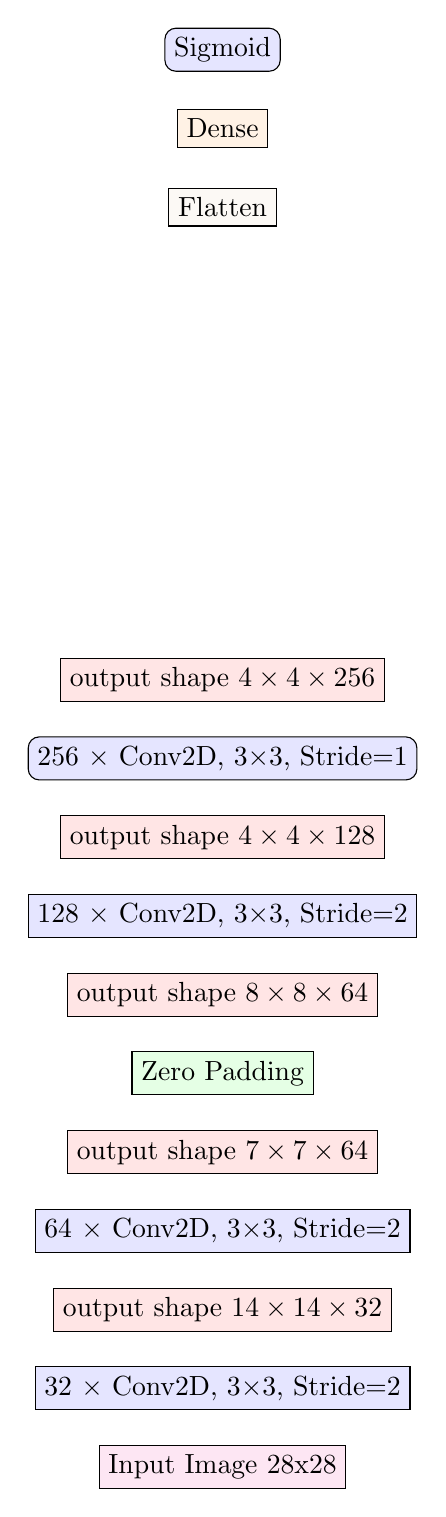
\begin{tikzpicture}
\tikzstyle{convlayer2} = [rectangle, rounded corners, fill=blue!10,draw=black]
\tikzstyle{convlayer1} = [rectangle, fill=blue!10, draw=black]
\tikzstyle{zeropadding} = [rectangle, fill=green!10, draw=black]
\tikzstyle{outputshape} = [rectangle, fill=red!10, draw=black]
\tikzstyle{dropout} = [rectangle, fill=black!5, draw=black]
\tikzstyle{flatten} = [rectangle, fill=brown!5, draw=black]
\tikzstyle{optimizer} = [rectangle, fill=purple!5, draw=black]
\tikzstyle{loss} = [rectanble, fill=cyan!10, draw=black]
\tikzstyle{dense} = [rectangle, fill=orange!10, draw=black]
\tikzstyle{image} = [rectangle, fill=magenta!10, draw=black]

\node(inputImage) [image] at (0,0) {Input Image 28x28};
\node(convLayer1) [convlayer1] at (0,1) {32 $\times$ Conv2D, 3$\times$3, Stride=2};
\node(output1) [outputshape] at (0,2) {output shape $14 \times 14 \times 32$};
\node(convLayer2) [convlayer1] at (0, 3) {64 $\times$ Conv2D, 3$\times$3, Stride=2};
\node(output2) [outputshape] at (0,4) {output shape $7 \times 7 \times 64$};
\node(zeropad) [zeropadding] at (0,5) {Zero Padding};
\node(output3) [outputshape] at (0,6) {output shape $8 \times 8 \times 64$};
\node(convLayer3) [convlayer1] at (0, 7) {128 $\times$ Conv2D, 3$\times$3, Stride=2};
\node(output3) [outputshape] at (0,8) {output shape $4 \times 4 \times 128$};
\node(convLayer4) [convlayer2] at (0, 9) {256 $\times$ Conv2D, 3$\times$3, Stride=1};
\node(output4) [outputshape] at (0,10) {output shape $4 \times 4 \times 256$};

\node[flatten] at (0,16) {Flatten};
\node[dense] at (0,17) {Dense};
\node[convlayer2] at (0,18) {Sigmoid};
\end{tikzpicture}
\caption{Discriminator Architecture}
\label{discAcc}
\end{figure}


\section{Experiments}
\section{Conclusions}
In this work we extend the GAN framework to include
multiple generators and discriminators.  We start with a typical GAN as the
basis for a chain of GAN's.  We then use the output of the first GAN as 
input to a subsequent GAN, instead of noise vectors that Goodfellow et al.
\cite{gan}, and other research typically employs.  We also include the output of
the previous discriminator's output as input for the generator.  We extend this
chain of GAN's to 6 iterations and find empirically that successive discriminators 
are capable of higher accuracy.   

Future work: formal justification of result. Try different GAN architectures.
Explore using different datasets as inputs for different iterations.
\section*{References}

Please number citations consecutively within brackets \cite{b1}. The 
sentence punctuation follows the bracket \cite{b2}. Refer simply to the reference 
number, as in \cite{b3}---do not use ``Ref. \cite{b3}'' or ``reference \cite{b3}'' except at 
the beginning of a sentence: ``Reference \cite{b3} was the first $\ldots$''

Number footnotes separately in superscripts. Place the actual footnote at 
the bottom of the column in which it was cited. Do not put footnotes in the 
abstract or reference list. Use letters for table footnotes.

Unless there are six authors or more give all authors' names; do not use 
``et al.''. Papers that have not been published, even if they have been 
submitted for publication, should be cited as ``unpublished'' \cite{b4}. Papers 
that have been accepted for publication should be cited as ``in press'' \cite{b5}. 
Capitalize only the first word in a paper title, except for proper nouns and 
element symbols.

For papers published in translation journals, please give the English 
citation first, followed by the original foreign-language citation \cite{b6}.

\begin{thebibliography}{00}
\bibitem{b1} G. Eason, B. Noble, and I. N. Sneddon, ``On certain integrals of Lipschitz-Hankel type involving products of Bessel functions,'' Phil. Trans. Roy. Soc. London, vol. A247, pp. 529--551, April 1955.
\bibitem{b2} J. Clerk Maxwell, A Treatise on Electricity and Magnetism, 3rd ed., vol. 2. Oxford: Clarendon, 1892, pp.68--73.
\bibitem{b3} I. S. Jacobs and C. P. Bean, ``Fine particles, thin films and exchange anisotropy,'' in Magnetism, vol. III, G. T. Rado and H. Suhl, Eds. New York: Academic, 1963, pp. 271--350.
\bibitem{b4} K. Elissa, ``Title of paper if known,'' unpublished.
\bibitem{b5} R. Nicole, ``Title of paper with only first word capitalized,'' J. Name Stand. Abbrev., in press.
\bibitem{b6} Y. Yorozu, M. Hirano, K. Oka, and Y. Tagawa, ``Electron spectroscopy studies on magneto-optical media and plastic substrate interface,'' IEEE Transl. J. Magn. Japan, vol. 2, pp. 740--741, August 1987 [Digests 9th Annual Conf. Magnetics Japan, p. 301, 1982].
\bibitem{b7} M. Young, The Technical Writer's Handbook. Mill Valley, CA: University Science, 1989.
\end{thebibliography}
\vspace{12pt}
\color{red}
IEEE conference templates contain guidance text for composing and formatting conference papers. Please ensure that all template text is removed from your conference paper prior to submission to the conference. Failure to remove the template text from your paper may result in your paper not being published.

\end{document}
